

\subsection{Miglioramento dell'efficienza con i Suffix Link}

Un primo miglioramento lo si ottiene utilizzando i \textbf{suffix link}, ovvero un collegamento tra due nodi espliciti dell'albero \textit{u} e $ s(u) $ tali che l'etichetta di $ u $ sia $ x\alpha $ e l'etichetta di $ s(u) $ sia $ \alpha $, in altre parole c'è un suffix link se l'etichetta di $ u $ è uguale all'etichetta di $ s(u) $ preceduta da un carattere qualsiasi (Fig \ref{asdasdasd2}).

\begin{figure}[htbp]
	\centering
	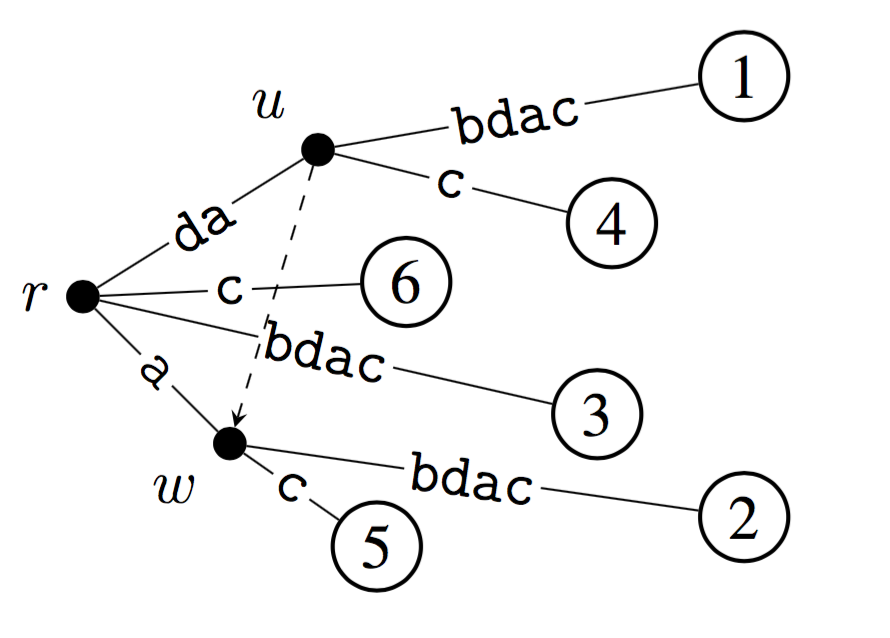
\includegraphics[width=.4\textwidth]{./notes/immagini/l22-fig1.png}
	\caption{In questo caso $\alpha=a$ e $x=d$}\label{asdasdasd2}
\end{figure}

Così facendo durante la costruzione dell'albero, quando viene esteso il cammino ad una foglia, posso tornare indietro fino a che non trovo un nodo esplicito con un suffix link e posso riprendere la costruzione dell'albero a partire dal nodo collegato.

Per ogni albero implicito $ I_i $, ogni nodo esplicito ha un suffix link uscente (\textbf{Lemma 5.4}), perché se durante la fase \textit{i}-esima per estendere il suffisso $ S[j,i] $, viene creato un nuovo nodo non foglia con etichetta $ x\alpha $ ($x\alpha$ prefisso di $ S[j,i] $) allora:

\begin{itemize}
	\item o nell'albero corrente esiste già un nodo interno esplicito con etichetta $\alpha$
	\item oppure tale nodo verrà creato immediatamente dopo con l'estensione del suffisso successivo $ S[j+1,i] $
\end{itemize}

Questo perché un nuovo nodo interno esplicito \textit{v} con etichetta $ S[j,i] = x\alpha $ viene creato soltanto se il suffisso $ S[j,i] $ viene esteso con il caso 2, quando nell'albero corrente il cammino $ S[j,i] $ termina in un nodo interno implicito e tale cammino continua con un carattere \textit{c} diverso da $S[i+1]$.

Quindi nell'albero corrente c'è anche il cammino di etichetta $S[j+1,i] = \alpha$ che ha una continuazione che inizia con il carattere \textit{c}.

Dunque il nodo $ w $ con etichetta $ S[j+1, i]  = \alpha$ è un nodo interno che può essere esplicito o implicito. Se è esplicito $w = s(v)$ altrimenti, il cammino di etichetta $ S[j+1, i] = \alpha $ che termina nel nodo \textit{w} può continuare solo con \textit{c} e quindi nel passo successivo l'estensione del suffisso $ S[j+1,i] $ sostituisce il nodo implicito con un nodo esplicito per cui $s(v) = w$.

Inoltre (\textbf{Corollario 5.5}), nell'algoritmo di Ukkonen, ogni nodo interno esplicito creato durante l'estensione di un suffisso ha sicuramente un suffix link da esso uscente dopo che sia stato esteso anche un il suffisso successivo.

Questo si dimostra per induzione. Per $ I_0 $ la cosa è banalmente vera perché è presente solo un nodo interno esplicito e la radice non viene creata estendendo un suffisso.

Supponendo quindi che al termine della fase $(i-1)$-esima ci siano tutti i suffix link, per il lemma precedente, se viene creato un nuovo nodo \textit{v} estendendo $ S[j,i] $, il nodo $ s(v) $ viene trovato o creato durante l'estensione del suffisso successivo $ S[j+1,i] $. Siccome l'estensione dell'ultimo suffisso $ S[i+1,i] $ non aggiunge nodi interni, alla fine della fase $ i $-esima, tutti i nodi interni espliciti hanno il loro suffix link.

In altre parole, in ogni albero dei suffissi impliciti $ I_i $, se un nodo interno esplicito ha etichetta di cammino $ x\alpha $ esiste anche un nodo interno esplicito di etichetta $\alpha$.

\subsubsection{Costruzione dell'albero utilizzando i suffix link}

Nella fase di costruzione dell'albero $ I_{i+1} $ (fase $ i $-esima), l'algoritmo di Ukkonen cerca i nodi in cui terminano i suffissi $ S[j,i] $ per estenderli con il carattere $ S[i+1] $ (Nella fase $i$-esima viene esteso l'albero implicito $I_i$ per ottenere l'albero implicito $_{i+1}$).

Il cammino relativo al suffisso $ S[1,i] $ sarà sempre presente e terminerà ogni volta in una foglia numerata, quindi questo può essere aggiornato sempre in tempo costante utilizzando il caso 1 e memorizzando un puntatore alla foglia.

Supponiamo di dover estendere un suffisso successivo $ S[j,i] $, uguale a quello precedente $ S[j-1,i] $ privato del primo carattere ($S[j-1,i] = x\alpha, S[j,i]= \alpha$, con $\alpha$ eventualmente nulla).

Sia \textit{v} l'ultimo nodo esplicito del cammino $ S[j-1,i] $, \textit{v} può essere la radice oppure un nodo interno di $ I_i $.

A questo punto, l'algoritmo per estendere il suffisso $ S[j,i] $ deve cercare nell'albero corrente il nodo con etichetta $ S[j,i] $.

Se \textit{v} è la radice, l'algoritmo si comporta come la versione ingenua e cerca il nodo a partire da essa.
Se invece \textit{v} è un nodo interno, per il corollario precedente, \textit{v} ha un suffix link $ s(v) $ e dato che l'etichetta di \textit{v} è un prefisso di $ x\alpha $, l'etichetta di $ s(v) $ è un prefisso di $\alpha$ e quindi per cercare il nodo con etichetta $ \alpha $ è possibile partire da $ s(v) $.

Più in dettaglio, l'estensione del suffisso $ S[j-1,i] $ avviene come segue:

\begin{enumerate}
	\item Sia $\beta$ l'etichetta del nodo $ s(v) $ e $ S[j,i] = \alpha = \beta\gamma $
	\item Per trovare la fine di $ S[j,i] = \alpha $ si parte da dove finisce $ S[j-1,i] = x\beta\gamma $ e si torna indietro al nodo \textit{v}.
	\item Si segue il suffix link per arrivare a $s(v)$ che ha $\beta$ come etichetta
	\item Si scende il cammino etichettato $\gamma$
	\item Alla fine di questo cammino c'è il nodo con etichetta $\alpha$, che può essere esteso con uno dei 3 casi.
\end{enumerate}

Come esempio vedi la figura \ref{sadefe2}

\begin{figure}[htbp]
	\centering
	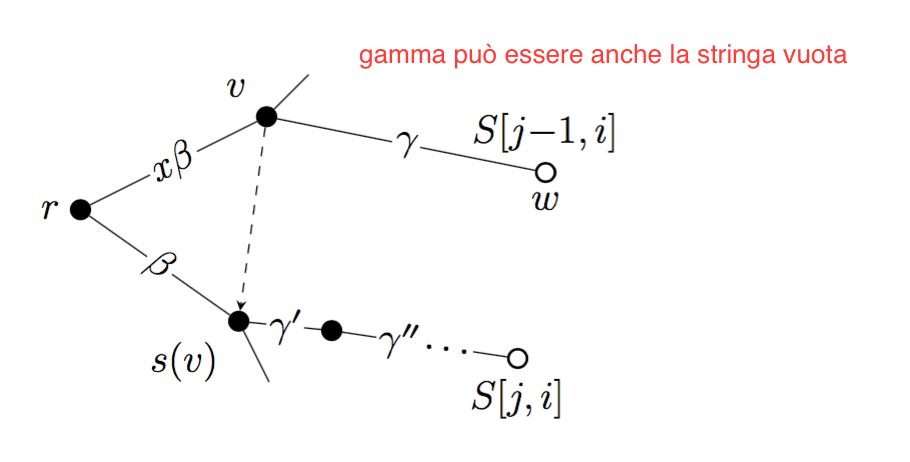
\includegraphics[width=.7\textwidth]{./notes/immagini/l22-fig3.png}
	\caption{La ricerca del suffisso $ S[j,i] $. Si risale, dal nodo con etichetta $ S[j-1,i] = x\alpha = x\beta\gamma $, per al più un arco $\gamma$ fino al nodo $ v $ di etichetta $ x\beta $; ci si muove quindi in $ s(v) $ utilizzando il suffix link e infine si scende il cammino cercando l'arco etichettato $\gamma = \gamma'\gamma''$ per arrivare al nodo di etichetta $ S[j,i] = \beta\gamma =\alpha$.}\label{sadefe2}
\end{figure}

Combinando il tutto l'algoritmo per l'estensione di un suffisso diventa:

\begin{enumerate}
	\item Partendo dal noto $ w $ dove termina il suffisso $ S[j,i] $ e risalendo verso la radice, cerca il primo nodo esplicito \textit{v} che o ha un suffix link oppure è la radice. Per i corollari precedenti richiede di risalire al massimo di un solo arco.
	
	Sia $\gamma$ l'etichetta, eventualmente nulla, del cammino dal nodo \textit{v} al nodo \textit{w}.
	
	\item Se \textit{v} non è la radice spostati su  $s(v)$ usando il suffix link e quindi discendi seguendo il cammino individuato dalla stringa $ \gamma $.
	
	Se \textit{v} è la radice segui il cammino individuato dalla stringa $ S[j+1,i] $ come per l'algoritmo ingenuo.
	
	\item Estendi il suffisso $ S[j+1,i] $ usando il caso appropriato.
	
	\item Se il nodo \textit{w} è un nodo interno esplicito creato durante l'estensione del suffisso precedente $S[j,i]$ (usando il caso 2), per il lemma 5.4 la stringa $ S[j+1,i] $ deve terminare in un nodo $ s(w) $ esplicito dopo l'estensione di $ S[j+1,i] $. In questo caso metti un suffix link da $ w $ a $ s(w) $
\end{enumerate}

Inoltre, mantenendo un puntatore alla foglia relativa al suffisso più lungo $ S=[1,i] $, la prima estensione della fase \textit{i}-esima non richiede alcuna ricerca e può essere fatta direttamente con il caso 1.

Nonostante ciò la complessità asintotica nel caso pessimo, con una stringa composta da tutti caratteri diversi, non migliora e risulta essere $ O(n^3) $.

\subsubsection{Skip - count}

Durante il secondo passo l'algoritmo discende dal nodo $s(v)$ al cammino di etichetta $\gamma$ e se questo viene fatto normalmente richiede un tempo proporzionale alla lunghezza di $\gamma$.

Sia $g = |\gamma|$ la lunghezza della stringa $\gamma$. Sappiamo che esiste un cammino etichettato con $\gamma$, che può essere anche nullo.

Se $g = 0$, il nodo $s(v)$ è proprio il nodo d'interesse, altrimenti, siccome tutti gli archi uscenti da $s(v)$ hanno etichette che iniziano con caratteri distinti, la scelta dell'arco lungo cui scendere richiede soltanto il confronto con il primo carattere di $\gamma$.

Sia $b$ la lunghezza dell'arco $\beta$ prescelto, tale lunghezza può essere memorizzata assieme all'etichetta.

\begin{itemize}
\item Se $b \leq g$ l'algoritmo non deve controllare nessun altro carattere di $\beta$, perché $\beta$ è certamente uguale al prefisso di $\gamma$ di lunghezza $b$, ossia $\gamma = \beta\gamma'$. L'algoritmo si sposta quindi direttamente sul nodo finale dell'arco prescelto per continuare la ricerca del cammino etichettato $\gamma'$.
\item Se $b > g$ il cammino etichettato $\gamma$ termina nel nodo implicito $g$-esimo di tale arco.
\end{itemize}

Assumendo quindi costante la dimensione dell'alfabeto, ogni spostamento da un nodo esplicito ad un altro nodo lungo il cammino etichettato $\gamma$ richiede un tempo costante.

Il \textbf{livello} $l(v)$ di un nodo esplicito \textit{v} è definito come il numero di archi del cammino dalla radice a \textit{v} o, equivalentemente, come il numero di nodi espliciti che precedono \textit{v} in tale cammino.

Si ha quindi che durante l'esecuzione dell'algoritmo di Ukkonen, viene attraversato un suffix link da $v$ a $s(v)$, vale il \textbf{Lemma 5.7}:

$$
l\big(s(v)\big) \geq l\big(v\big) -1
$$

Questo perché ogni nodo esplicito che precede \textit{v}, esclusa la radice, ha un suffix link che punto ad un nodo che precede $s(v)$. Infatti se l'etichetta del cammino di $v$ è $x\beta$, prefisso del suffisso precedente $S[j,i]$, l'etichetta di cammino di $s(v)$ è $\beta$, prefisso del suffisso $S[j+1,i]$.

Usando quindi lo skip/count, ogni fase dell'algoritmo di Ukkonen richiede tempo $O(n)$.

Infatti, nella fase $i$-esima vengono effettuate $i+1$ estensioni. In ogni estensione l'algoritmo risale al più di un solo arco per trovare il nodo con suffix link, attraversa il suffix link, discende un certo numero di archi e quindi applica uno dei tre casi per l'estensione del suffisso ed eventualmente aggiunge un suffix link. Tutte queste operazioni possono essere fatte in tempo costante, tranne la discesa che dipende dal numero di archi percorsi.

Consideriamo come varia il livello corrente $l$ durante una fase, ossia il livello dell'ultimo nodo esplicito visitato dall'algoritmo.
L'estensione del primo suffisso non modifica $l$ perché applica il caso 1 sul suffisso più lungo.

Ad ogni estensione successiva, \textit{l} diminuisce al più di una unità nella risalita, diminuisce al più di una unità attraversando il suffix link ed aumenta di una unità ogni volta che si discende un arco. Quindi durante l'intera fase \textit{l} può diminuire al più $2i$ volte.

Siccome $l$ rimane sempre $\leq i$, ogni arco ha un'etichetta di almeno un carattere e le etichette sono lunghe al massimo $i$), esso non può aumentare più di $3i$ volte e quindi il numero totale di archi discesi in tutta la fase è al più $3i = O(n)$.

Ricapitolando:
\begin{itemize}
	\item Estendere un suffisso con uno dei 3 casi viene fatto in tempo costante, l'importante è trovare cammino dell'albero da estendere
	\item Utilizzano il suffix-link e lo skip/count ogni fase, ovvero l'estensione dell'albero dei suffissi $I_i$ per la stringa $S[1,i]$ nell'albero dei suffissi $I_{i+1}$ per la stringa $S[1,i+1]$, può essere fatta in $O(n)$, questo perché entrambi gli accorgimenti velocizzano la ricerca dei cammini.
	\item Per ottenere l'albero dei suffissi per la stringa sono necessari $n$ fasi.
\end{itemize}

In tutto si ha una complessità di $O(n^2)$.

\subsubsection{Il problema dello spazio}

Al momento l'albero dei suffissi può richiedere uno spazio $O(n^2)$ e ovviamente non può essere costruito in $O(n)$.

Questa occupazione in spazio deriva dal fatto che, anche se i nodi dell'albero non possono essere più di $2n-1$, la somma delle lunghezze delle etichette può richiedere $O(n^2)$. I nodi dell'albero sono le $n$ foglie ed al più $n-1$ nodi interni (perché ogni nodo ha almeno due figli). Nel caso di una stringa con tutti i caratteri distinti, l'albero dei suffissi è costituito soltanto dalla radice e dalle $n$ foglie e la somma delle lunghezze delle etichette è $\sum_{i=1}^n i = O(n^2)$.

La soluzioni è quindi quella di rappresentare l'etichetta di un arco con una coppia di indici $(p,q)$ tale che l'etichetta sia $\beta = S[p,q]$, resta inoltre possibile calcolare la lunghezza per effettuare lo skip count con $b = q -p+1$.

Utilizzando le coppie di indici lo spazio richiesto per memorizzare un'etichetta diventa costante.

\subsubsection{Limitazione delle fasi}

Si può osservare che non appena in una fase viene applicato il caso 3, questo viene applicato anche a tutte le successive estensioni della stessa fase.

Questo perché, se viene applicato il caso 3 per l'estensione del suffisso $S[j,i]$ significa che il suffisso $S[j,i+1]$ è già presente nell'albero corrente e quindi sono presenti anche tutti i suffissi successivi da $S[j+1,i+1]$ ad $S[i+1,i+1]$.
Ovvero quando viene applicato il caso 3 vuol dire che all'interno dell'albero è già stato inserito il suffisso $S[j',i+1]$ che ha come prefisso $S[j,i+1]$ per $j' < j$.

Si ha quindi che non appena viene applicato il caso 3, la fase di estensione dell'albero può terminare.

Inoltre, se ad un certo punto dell'algoritmo di Ukkonen viene creata una foglia etichettata \textit{j} per inserire il suffisso $S[j,i+1]$ (caso 2) tale foglia rimane una foglia in tutti i successivi alberi costruiti dall'algoritmo, questo perché l'algoritmo non estende mai un cammino oltre la foglia che lo termina. Quindi tutte le estensioni successive del suffisso associato a tale foglia verranno sempre fatte applicando il caso 1.

L'esecuzione di una fase dell'algoritmo quindi procede sempre secondo un determinato schema:

\begin{enumerate}
	\item La foglia 1 viene costruita nella fase 1, quindi ogni fase inizia con un'estensione che usa il caso 1.
	\item Vengono poi eseguite delle estensioni che usano i casi 1 e 2
	\item Termina non appena viene eseguito il primo caso 3.
\end{enumerate}

Sia $j_{i-1}$ l'ultima estensione che usa i casi 1 o 2 nella fase $(i-1)$-esima. Siccome ogni applicazione del caso 2 crea una nuova foglia, alle prime $j_{i-1}$ estensione della fase successiva si applica il caso 1, per quanto precedentemente osservato.

Dunque per la fase successiva si avrà $j_i \geq j_{i-1}$ e questo ci suggerisce di cercare un trucco che faccia evitare, nella fase successiva, le prime $j_{i-1}$ estensioni che utilizzano il caso 1.

Si può osservare che il caso 1 si limita ad aggiungere all'etichetta dell'arco che termina nella foglia di etichetta $S[j,i]$ il carattere $S[i+1]$.
Quando viene creata una foglia con il caso 2 nella fase $i$-esima all'arco che termina nella foglia viene assegnato solamente il carattere $S[i+1]$ come etichetta. 
Da quel momento in poi l'etichetta verrà via via allungata di un carattere per ogni fase, fino a diventare $S[i+1,n]$.

Si può quindi assegnare, alla creazione della foglia come caso 2, l'etichetta $S[i+1,n]$, sempre se la stringa è nota a priori. Se questo non lo è come coppia che identifica l'etichetta è possibile utilizzare il valore $(i+1,e)$.

Così facendo le prime $j_{i-1}$ estensioni nella fase $i$-esima, non richiedono alcuna operazione e possono essere saltate, iniziando all'estensione $(j_{i-1}+1)$-esima. La fase $i$-esima inizia quindi con l'estensione $j = i_{j-1}+1$ e termina con la prima estensione che usa il caso 3 oppure quando tutti i suffissi sono stati estesi (in questo caso si ha $j = i+2$).

Il valore per la fase successiva risulta essere $j_i = j-1$, ovvero l'ultima posizione che non è stata estesa con il caso 3.

\begin{figure}[htbp]
	\centering
	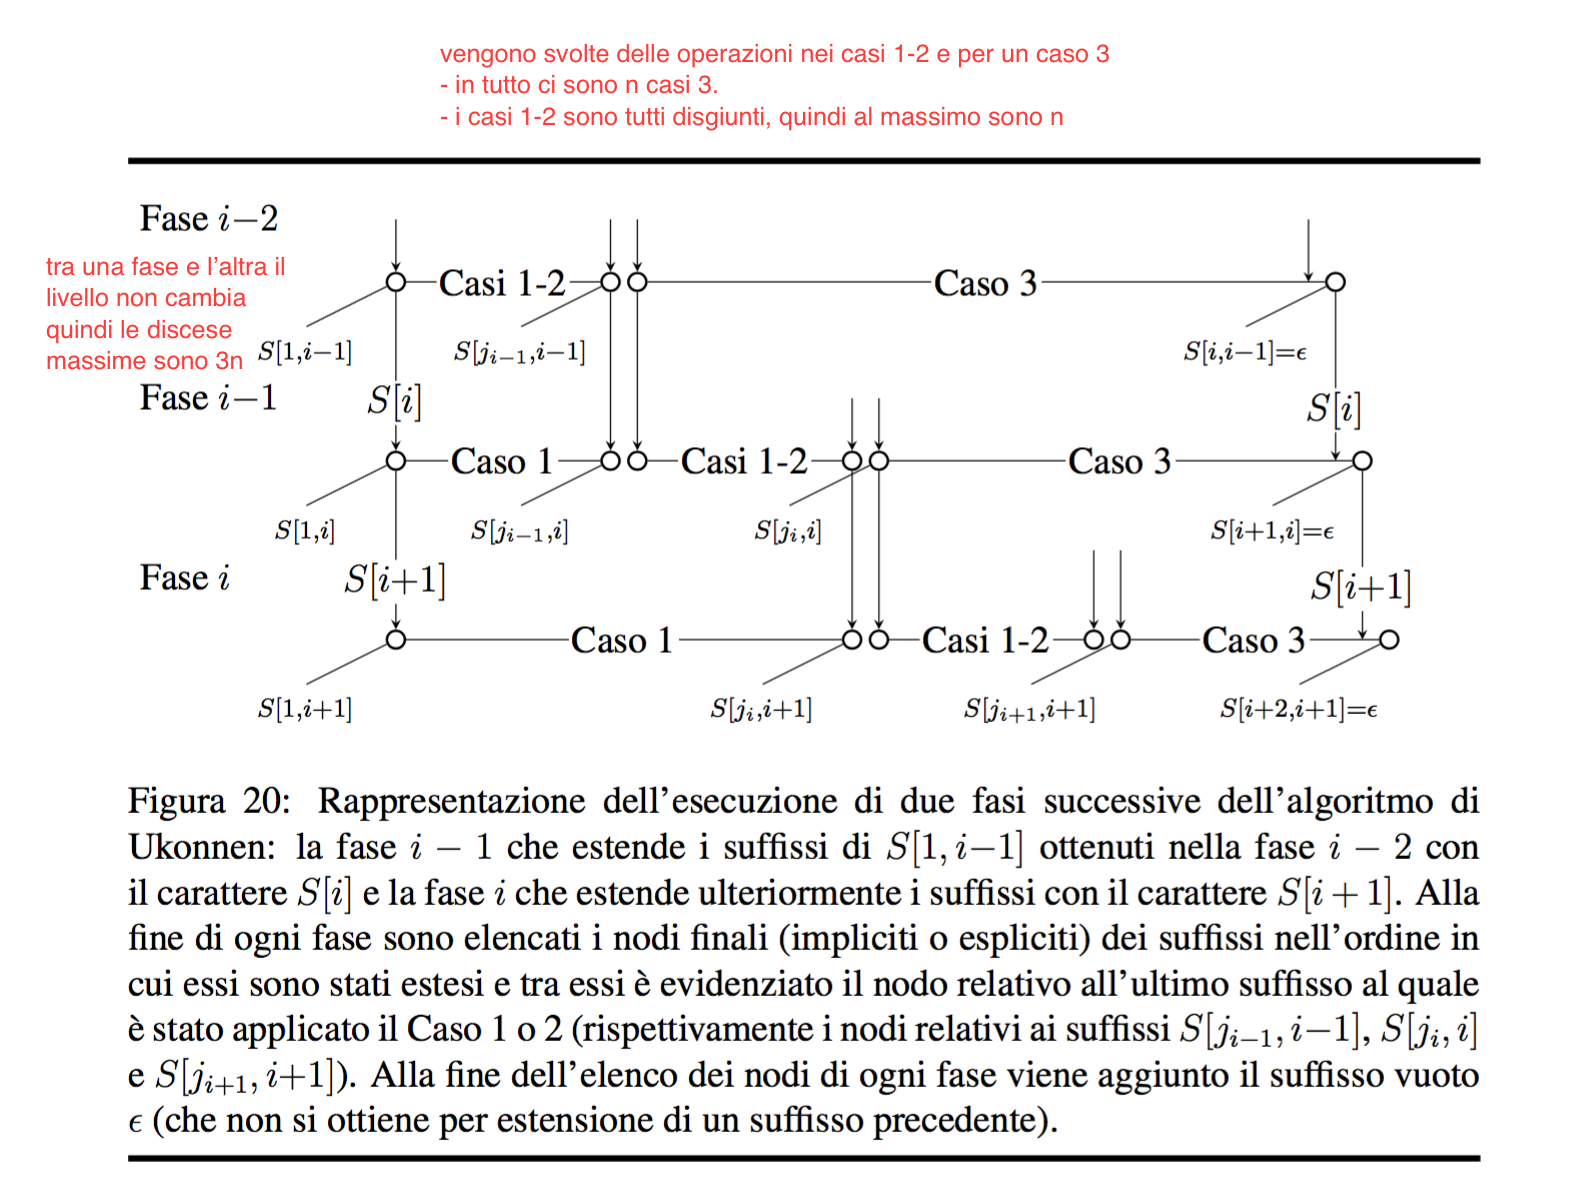
\includegraphics[width=.9\textwidth]{./notes/immagini/l22-fig8.png}
\end{figure}

\paragraph{Dimostrazione del tempo di esecuzione costante}

Se $S[j*, i-1]$ è l'ultimo suffisso esteso nella fase $(i-1)$-esima, la fase $i$-esima inizia con l'estensione del suffisso $S[j*,i]$. Dunque soltanto il suffisso $j*$-esimo viene esteso sia nella fase $(i-1)$-esima che nella fase $i$-esima.

Siccome gli indici $j$ dei suffissi sono tutti minori o uguali ad $n$ e le fasi sono $n$, in totale vengono eseguite al più $2n$ estensioni durante tutta l'esecuzione dell'algoritmo, con ogni estensione che richiede un tempo costante più un tempo proporzionale al numero di archi discesi nella ricerca di $\gamma$, che è un $O(n)$.

Siccome la fase $i$-esima inizia con il suffisso $j*$-esimo in cui è avvenuta l'ultima estensione della fase precedente, il livello corrente non cambia passando da una fase alla successiva (anche nel caso in cui $j_{i-1}=i$, il livello corrente quando si è esteso l'ultimo suffisso $S[i,i-1] = \epsilon$ nella fase $(i-1)$-esima era 0, uguale al livello corrente quando si estende il primo suffisso $S[i+1,i] = \epsilon$ nella fase $i$-esima).

Dunque il fatto che il livello corrente non diminuisca mai più di due volte vale sia all'interno di una singola fase che per tutto l'algoritmo e siccome il livello rimane sempre compreso tra 0 e $n$, il numero di archi discesi durante tutta l'esecuzione dell'algoritmo deve essere minore o uguale a $3n$.

Questo perché nella stessa fase, per quanto precedentemente dimostrato, il livello diminuisce al più di due volte e tra una fase e l'altra il livello non cambia.

Siccome durante tutta l'esecuzione dell'algoritmo vengono eseguite al più $2n$ estensioni ciascuna delle quali richiede un tempo costante più un tempo proporzionale agli archi discesi e il numero totale di archi discesi è minore o uguale a $3n$ si può concludere che l'algoritmo richiede un tempo $O(n)$. Questo perché nelle $2n$ estensioni vengono discesi al massimo $3n$ archi, si ha quindi come complessità $O(2n)+ O(3n) = O(n)$.

Se la lunghezza della stringa non è nota a priori, una volta completata l'esecuzione è necessario andare a correggere le etichette delle foglie.

L'algoritmo di Ukkonen quindi, costruisce on-line l'albero dei suffissi di una stringa di lunghezza $n$ in $O(n)$.